\chapter{文本匹配算法的并行实现}

在前面的章节中,本文已经介绍了基于强化学习的文本匹配算法,实验证明该算法可以在多个评价指标上都有效的提高文本匹配算法的精度。但是由于蒙特卡洛树搜索耗时极长,因此对必须算法进行并行化以有效提高训练和推断速度。本章基于第\ref{chap:Zero}章所提出的算法,介绍了该算法的并行实现。

\section{Tensorflow 介绍}
\label{sec:intro2tf}
本章所介绍的实现都是基于 Tensorflow\cite{Abadi2016TensorFlowAS} 开发的,因此首先对 Tensorflow 进行介绍。Tensorflow 是谷歌在2016开源的深度学习库,得到广泛关注,并迅速在计算机视觉、自然语言处理等等领域被工业界和学术界广泛使用。

Tensorflow 是一个强大的深度学习软件库,它支持任何可以被表示为数据流图的计算过程。通过对线程、队列和异步计算的支持,Tensorflow 可以在单机、多机、同构、异构等多种场景下运行,同时可以根据计算需要,合理的分配运行节点的位置。

在 Tensorflow 中,一个数据流图的表示如图 \ref{fig:tensorflow_dep} 所示。图中的每个节点表示一个算子,边表示不同算子之间的数据交互。

\begin{figure}[!htbp]
    \centering
    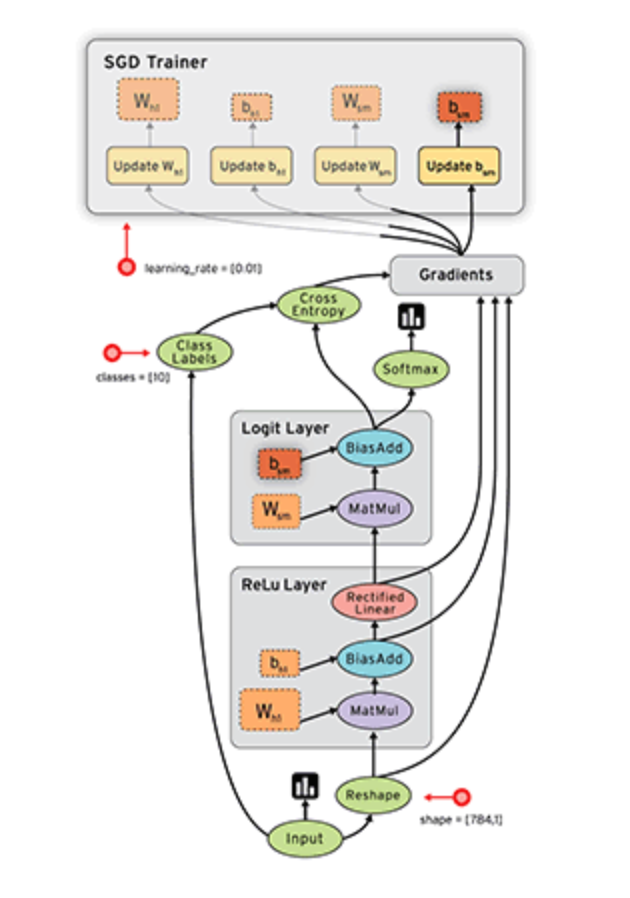
\includegraphics[width=0.5\textwidth]{data_flow}
    \bicaption{TensorFlow 数据流图}{Tensorflow data flow}
    \label{fig:tensorflow_dep}
\end{figure}

数据流图中包括以下几个主要元素:

1. 算子。算子是 Tensorflow 中基本的数据处理单元,算子可以有多个输入和多个输出。Tensorflow 中的算子包括元素运算、矩阵运算、数值生成以及 IO 交互。例如矩阵乘法就是一个矩阵运算的算子。每个算子都在至少一个计算设备上实现,运行时 Tensorflow 会自己确定算子实际运行的计算设备。

2. 张量。张量是计算图中的边表示不同算子之间的数据交互的载体。在实际计算过程中,张量往往是一个或多个高为矩阵。 Tensorflow 中的张量仅仅保存对数据的访问接口,所有的张量都是在运行时动态分配的。

3. 变量。变量时计算图中的可变节点。例如在神经网络训练时,每次迭代结束后都会对参数进行更新,这些参数在 Tensorflow 中即被表示为变量。

4. 会话。所有计算图的计算都必须在会话中进行。会话主要负责计算设备的初始化、内存分配,以及在运行前对计算图的处理。对计算图的处理主要包括重复操作的合并、算子的计算设备分配等等。

\section{系统架构}
本小节对算法\ref{alg:Train} 的过程进行分析,并根据本文所提出的算法特点确定适合于本文算法的架构。

在 \ref{sec:intro2tf}节中,我们介绍了 Tensorflow 的数据流图。目前大部分算法都可以被表示为数据流图的形式,因此可以直接使用 Tensorflow 运行。由于 Tensorflow 在运行前会先进行图裁剪等准备工作,因此批量化(batch)的数据处理可以大大减少会话中计算图处理的次数;同时由于 SSE、AVX 等 SIMD 指令集的存在,使得数值运算在大数据量场景下的效率大大提升,因此批量化的数据处理得到了大部分深度学习库的广泛支持。

但是强化学习由于存在主体和环境的交互,不同主体在同一时刻 $t$ 所面对的环境和状态都不尽相同,大部分场景下环境和状态的矩阵表示甚至难以做到维数相同。这种复杂环境使得很难对不同的主体进行批量化处理;与此同时,主体在时刻 $t$ 的策略可能需要很长时间之后才可以从环境得到奖励,这种推断和更新的延迟很难通过计算图的形式进行呈现,因此Tensorflow 只能用于策略和价值网络的计算中,不能直接利用其计算图建模整个强化学习过程。

仔细观察 \ref{sec:MCTS_intro} 节中的蒙特卡罗树搜索算法,可以发现该算法可以被分为以下几个独立部分:

1. 节点选择以及节点评价。在节点选择时,我们从根节点 $s_R$ 开始以最大化上限置信区间为目标选择行动。在行动选择时,我们的计算目标只与当前节点的访问次数以及行动价值有关;在评价扩展时,我们需要根据当前节点的状态计算节点价值。他们的计算都只与当前节点有关,不会涉及到树的结构改变或者是节点更新;

2. 节点扩展以及节点更新。在节点评价结束后,如果当前节点为叶节点且当前节点的状态不在匹配矩阵的右下角,我们需要进行节点扩展;扩展结束后,需要根据本次搜索访问节点更新访问到的边。这两个操作均涉及到对蒙特卡罗树的更新,尤其是节点更新,需要改变的节点数量较大。

3. 策略计算。策略计算只与根节点 $s_R$ 的出边有关,但是和节点选择以及评价不同,策略计算的计算量很小。

这种情况下,很显然的方案是对3个独立部分进行分别处理,即对节点选择、节点评价以及策略计算进行并行处理,在节点扩展和节点更新时接受不同主体的状态,此时将数据按照本身的维度进行批量化处理(在本文的算法中即按照历史路径的长度进行批量化处理),利用 Tensorflow 进行计算。

\begin{figure}[!htbp]
    \centering
    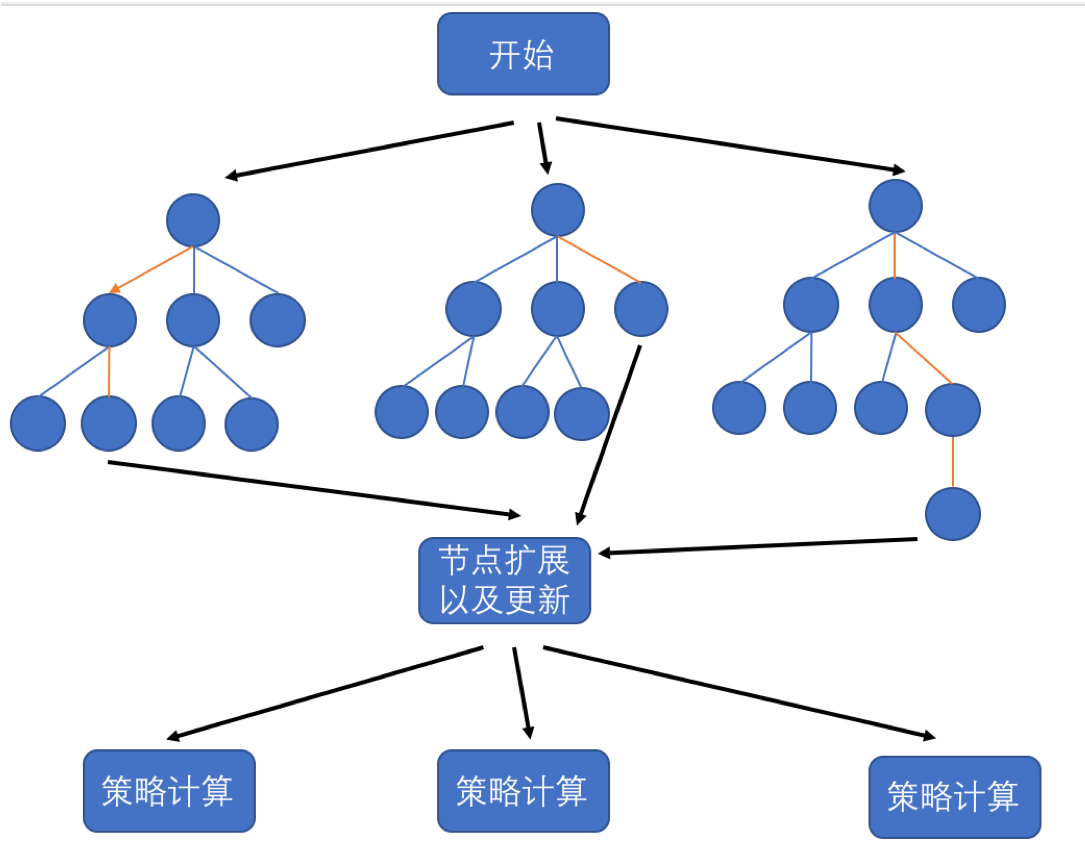
\includegraphics[width=0.5\textwidth]{wrong_sta}
    \bicaption{蒙特卡罗树搜索算法的批量化并行化方案}{Parallel batch implement of MCTS}
    \label{fig:tensorflow_dep}
\end{figure}

显然在节点扩展以及节点更新模块需要进行数据合并。如果使用这种方法,在节点选择和节点评价时并行选择就会成为很大的问题。在这里的并行有2种方法:

1. 在节点扩展以及节点更新时等待所有的树搜索完成。这种方案的实现简单,在整个搜索过程中都可以做到没有加锁和解锁的开销;但是由于需要等待所有树搜索完成,因此在时间上会造成极大的浪费;

2. 节点扩展以及节点更新时只等待部分树搜索完成。这种情况下存在多线程并发进行数据合并的可能性,因此需要引入互斥锁或者自旋锁进行线程同步。在表 \ref{tab:MCTS_runtime} 中,我们列出了在蒙特卡罗树搜索的各个主要耗时操作的时间。由于三个操作的耗时都与历史路径的长度有很大关系,因此没有列出具体数字,仅仅列出数量级以供参考。

\begin{table}[H]
    \bicaption{蒙特卡罗树搜索各个阶段耗时}{Time of each process in MCTS}
    \label{tab:MCTS_runtime}
    \centering
    \footnotesize% fontsize
    \setlength{\tabcolsep}{4pt}% column separation
    \renewcommand{\arraystretch}{1.2}%row space
    \begin{tabular}{cccc}
        \hline
        阶段 & 节点选择 & 数据拷贝 & 策略价值网络计算 \\
        \hline
        运行时间比例 & $1$ & $3.2451$ & $1342.3$ \\
        \hline
    \end{tabular}
\end{table}

从表中,我们可以发现节点选择的时间小于数据拷贝的时间。事实上,就运行时间来看,节点选择一般在1至3微秒,也就是说在1秒内,一个线程可以执行约上万次搜索,而每个线程在执行完一次搜索后,数据合并的时间是搜索时间的约3倍。这意味只要存在大于4个线程搜索,就至少一个线程在堵塞在线程同步上。在这种情况下会退化成第一种方案,而且由于加入了锁的同步开销,这种方案的表现只会差于第一种方案。

\begin{figure}[!htbp]
    \centering
    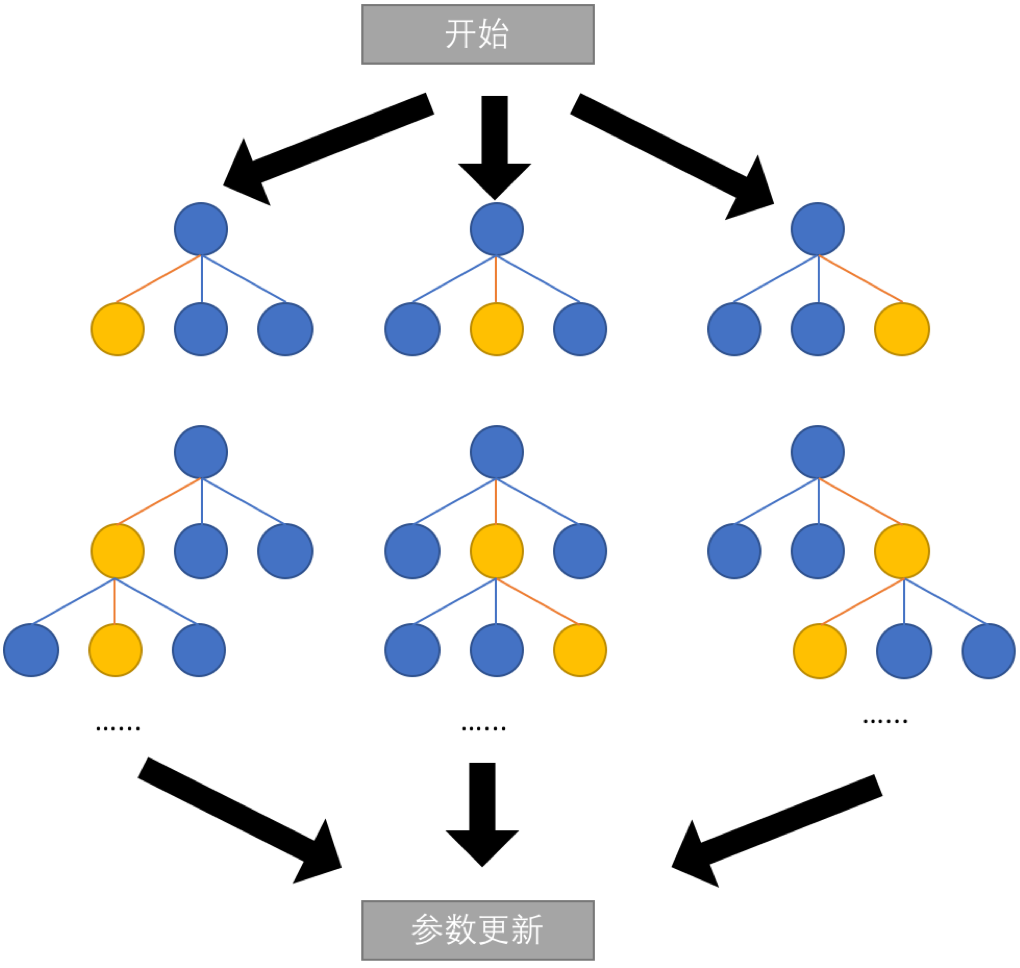
\includegraphics[width=0.5\textwidth]{parallel}
    \bicaption{蒙特卡罗树搜索算法的非批量化并行化方案}{Parallel non-batch implement of MCTS}
    \label{fig:tensorflow_para}
\end{figure}

根据上文的分析,我们在树搜索阶段进行参数合并进行计算是很难做到高效的。因此本文选择在树搜索阶段不进行参数合并;所有的参数合并只在策略和价值网络更新时进行。这种设计在树搜索的过程中完全避免了数据拷贝带来的加锁问题;但是与之相比导致策略价值网络的计算开销增加。虽然单线程的搜索时间增长,但是相比于前两种方案来说,增长仍然有限。

\section{蒙特卡罗树搜索并行实现}
基于前面的分析,本节介绍蒙特卡罗树搜索的并行实现。本节介绍的实现主要由 4 部分组成:蒙特卡罗树搜索、文本匹配模型、线程池以及内存池。

\begin{figure}[!htbp]
    \centering
    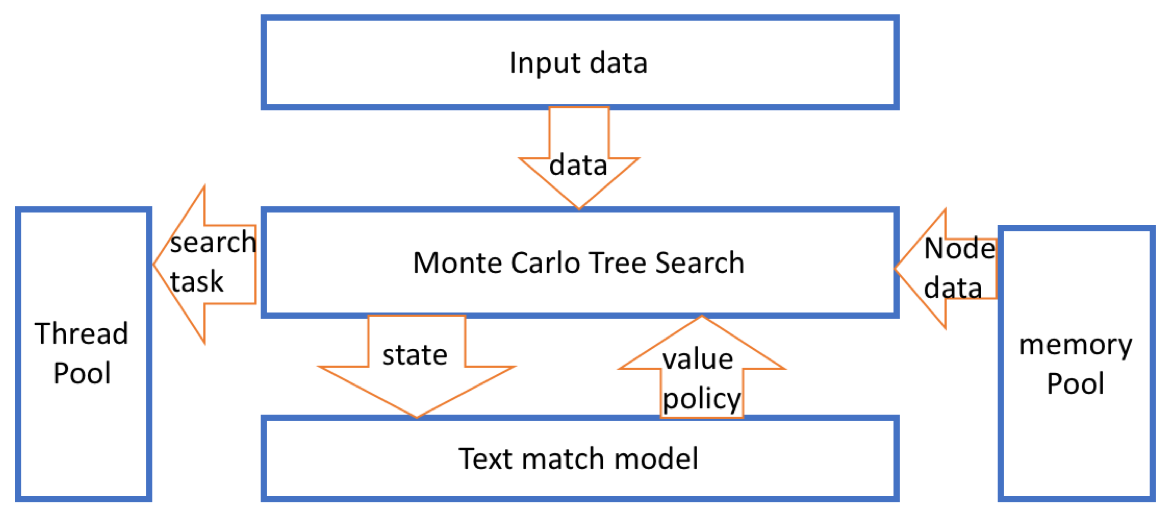
\includegraphics[width=0.5\textwidth]{para_arch}
    \bicaption{蒙特卡罗树搜索算法并行实现架构}{Architecture of parallel MCTS}
    \label{fig:tensorflow_para}
\end{figure}

其中蒙特卡罗树搜索是一个单线程的树搜索模块,主要负责树搜索的整体过程,包括选择,评价扩展,回溯更新以及策略计算,文本匹配模型即使用 Tensorflow 实现的第\ref{sec:MCTS_train}节所提出的文本匹配算法,线程池用于并行的任务处理,内存池用于节点的内存分配。因为文本匹配模型直接使用 Tensorflow 实现,所以本小节详细介绍其他三个模块的细节。

1. 内存池模块

在树搜索的过程我们会从根节点开始,一直遍历到叶节点,当遍历到叶节点时进行叶节点的扩展。由于蒙特卡罗树的深度极可能超过50,因此在栈上初始化所有的叶节点显然不现实。在堆上进行初始化时需要系统调用,这会浪费大量的时间用于内核态和用户态的切换。因此我们需要内存池减少系统花费在内存分配上的时间。

在蒙特卡罗树搜索的过程中,每个叶节点在初始化都是不会释放的,直到一次训练完成。因此就内存池来说,只会存在创建对象和清空内存池两个操作,不需要考虑内存池中创建对象的删除操作,因为不会存在单个对象的删除;同时由于节点的分配都是在叶节点扩展时,而每次叶节点的扩展都会生成3个新节点,因此节点的分配都是以3为单位。

本节所介绍的内存池由一个内存链表组成,链表中的每一个节点都指向一块固定大小的内存,内存大小由用户设置。为了避免一次分配3个节点时跨块分配判断的开销,内存池的大小会向 3 对齐。内存池内部保存一个当前所属链表节点的指针以及在当前内存块的偏移量。

内存池收到创建对象的请求时,首先检查当前内存块是否有剩余。如果当前内存块没有剩余,则开辟新的内存块,并根据新的内存块位置更新当前链表节点的指针以及偏移量。

内存池收到清除请求时,仅仅会重置当前链表节点的指针以及偏移量。即使是面对不同的数据,在树搜索过程中单棵树节点数量的方差也不会太大,因此保留已有的数据块可以减少数据块的分配和释放次数。

为了减少内存分配时不同线程之间的同步开销,我们没有设置全局的内存池,每个线程拥有自己的内存池。

2. 线程池模块

线程池模块主要用于处理蒙特卡罗树搜索的并行化调度。同内存池模块一样,由于线程池中每个线程都会进行一个样本的蒙特卡罗树搜索,因此在训练或者推断的过程中,线程池的任务是一次性添加的。由于样本之间没有交互,因此所有的搜索细节都可以放到单个线程中,也就是说像线程池中插入任务时,我们可以直接插入一个批量的任务。

本节所介绍的线程池由两部分组成:任务队列以及线程数组。每次当线程数组从当前队列中获取任务,运行直到当前队列中没有任务为止。由于当前队列每次加入任务时都需要进行加锁和解锁,这样在一次性加入大量任务的时候会有大量的锁调用开销。因此在添加任务时,我们直接将整个批次的任务添加到线程池中。由于在添加任务时,线程池的任务队列总是空的,因此我们直接修改线程池的任务队列的数据指针为添加任务列表的地址,这样可以减少任务拷贝的调用开销。

3. 蒙特卡罗树搜索模块

该模块主要由两部分组成:多叉树以及搜索算法。

多叉树上的每个节点都需要存储当前时刻的状态 $s$ 。根据前文的描述,我们所需要存储的状态包括历史路径和未来的词向量。在 $t$ 时刻,一个节点所需要存储的数据量为 $32\times(t+k)\times l_{word\_vec}$ 位。$k$ 表示向前看的但词个数, $l_{{word\_vec}}$ 表示词向量的维度,32 为浮点数的位数。这种情况下当句子对中有一个句子的长度过长时,会导致部分节点历史路径过长,单节点存储容量过大而导致内存无法装载全部树节点的情况出现。

为了降低单个子节点的内存消耗,我们只在树节点存储对应单词在句子中的位置,将单词和完整的句矩阵输入到 Tensorflow 。但是这样会导致我们每次都需要将完整的训练集句子作为输入,而 Tensorflow 在处理输入数据时同样需要进行数据拷贝。为了降低这些潜在开销,我们将训练集作为变量保存到了网络中,每轮训练开始前先将对应的 variable 节点中存储的数据更新为本轮的训练数据。这种情况下可以有效避免 Tensorflow 本身的数据拷贝开销,提供系统的运行效率。

蒙特卡罗树搜索的算法和算法 \ref{alg:TreeSearch} 中的表现基本一致,由于是单线程实现,因此不多做描述。在算法 \ref{alg:Train} 和算法\ref{alg:RLRank_MCTS} 中,在每次树搜索之后,我们根据当前树搜索的结果确定了下一步行动之后,会移动到新的节点,并将新节点作为根节点继续搜索。为了减少总搜索次数,我们对以前的树搜索结果进行了重用。即我们不会在新树上进行搜索,而是在上一次树搜索的结果之上进行。

\section{实验结果}
本节主要对本章设计的蒙特卡罗树搜索的并行实现进行性能测试,并对实验结果进行分析,以验证该实现的性能和功能是否达到了需求。由于目前没有针对蒙特卡罗树搜索的开源实现,因此本节的实验没有对比系统。
\subsection{实验设置}
本次实验所使用的服务器节点配置情况如表 \ref{tab:exp_machine} 所示:

\begin{table}[H]
    \bicaption{单服务器软硬件配置}{Server configuration}
    \label{tab:exp_machine}
    \centering
    \footnotesize% fontsize
    \setlength{\tabcolsep}{4pt}% column separation
    \renewcommand{\arraystretch}{1.2}%row space
    \begin{tabular}{|c|c|}
        \hline
        CPU型号 & Intel® Xeon® CPU E5-2420 0 @ 1.90GHz  \\
        \hline
        CPU核心数 & $2(\text{CPU}) \times 6(\text{核心数}) \times 2(\text{超线程}) = 24$ \\
        \hline
        内存 & 32G \\
        \hline
        操作系统 & CentOS Linux release 7.4.1708 \\
        \hline
        gcc版本 & 4.8.3\\
        \hline
        bazel版本 & 0.8.1 \\
        \hline
        Tensorflow版本 & 1.4.1\\
        \hline
    \end{tabular}{}
\end{table}

\subsection{多线程测试}
多线程测试主要是验证算法在多线程环境下能否达到较高的性能。多线程环境下的测试方法为:我们选择句子长度均为 10,词向量为 300,批处理大小为 1024 的数据,蒙特卡洛树搜索的搜索次数为50,在并发线程数在1到10的场景下进行了测试。测试结果如下:
\begin{figure}[!htbp]
    \centering
    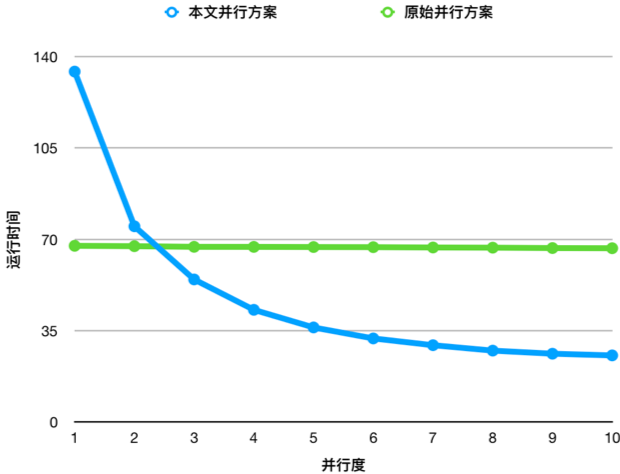
\includegraphics[width=0.8\textwidth]{para_lab}
    \bicaption{多线程加速比}{Multi-thread speed up ratio}
    \label{fig:para_lab}
\end{figure}
可以发现当线程数1到10之间是都会有加速效果,但是加速比是逐渐下降的,其中1到4线程场景下加速度大于0.8,相对较高。加速比下降的主要原因为:

1.多线程的同步开销。我们虽然对树搜索本身进行了并行,但是在模型更新阶段我们仍然需要从各个线程获得数据,在线程数量增加的情况下,不同线程竞争锁的概率会增加,进而导致同步开销增加;

2. 蒙特卡罗树搜索的线程和 Tensorflow 线程争夺CPU资源。为了能够并发的执行计算流图,Tensorflow 内部同样有一个线程池以进行计算图的并发执行。当我们将并发度设为10的情况下,Tensorflow 必须做到每个图只运行在一个线程上,这样才可以保证所有的线程不会争夺 CPU 资源。这显然不可能。

\section{本章小结}
本章在第\ref{chap:Zero}章提出算法的基础上进行了并行实现。

本章首先介绍了蒙特卡洛搜索树的不同并行实现方案,并针对于本文算法的场景进行分析。批量化计算虽然可以带来加速单个样本的训练和推断速度,但是由于数据拷贝时需要进行线程之间的同步,因此会极大拖慢系统整体的运行速度。本文提出的蒙特卡罗树搜索的完全并行方案极大的减少了线程间的同步开销。

第二部分根据第一部分的设计介绍了具体的实现。针对于蒙特卡罗树搜索的特殊场景,我们对进程池和内存池的设计进行了优化,同时对为了减少内存开销,简化了节点存储数据,避免了Tensorflow运行时的内存拷贝开销。

最后本文在多线程环境下对本章的实现进行了测试,事实证明,在线程数量较少时,本章所提出的并行设计可以获得较好的加速比;在并行度增加后,由于 Tensorflow 的线程干扰以及线程间同步开销的增加,加速比有所降低,但是仍然可以获得较高的加速效果。
